\documentclass{report}

\usepackage{listings}
\usepackage{color}
\usepackage{graphicx}
\usepackage{float}
\usepackage{amsmath}
\usepackage{subfig}
\usepackage{cite}
\usepackage{url}
\usepackage{amsmath}

\begin{document}

\title{3d Graphics - Sea seen from the beach}

\author{Jander Nascimento, 
\and Oleg Iegorov}

\maketitle

\section{Question 1}

\emph{Explain why rendering such a scene is very likely to produce
aliasing effects. Will the deformation of the sea surface due to waves
increase or tend to hide these visual problems?}

The aliasing effect happens when we try to sample a high resolution image\cite{iaow}, in case of long distance representation, due to the render limitation we cannot represent the detaild image, to overcome this issue a sampling is done to render far away cenarios, but sampling selects certain pixels for displaying, thus the representation becomes innacurate since a long distance pixels should be in matter of fact a composition (interpolation) of its neighbors.

In the Figure \ref{fig:aliasing} is shown one example of aliasing effect in long distances representation.

\begin{figure}[H]
		  \centering
		  \subfloat[Sampled image]{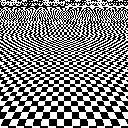
\includegraphics[width=0.4\textwidth]{image/alias01.png}\label{fig:sampled}}
		  \hspace{0.1cm}
		  \subfloat[Anti-aliased image]{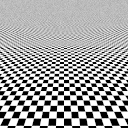
\includegraphics[width=0.4\textwidth]{image/alias02.png}\label{fig:antialiased}}
		  \caption{Aliasing effect}
		  \label{fig:aliasing}
\end{figure}

In the Figure \ref{fig:aliasing}, we are using a chessboard pattern as the texture for the ground, in the Figure \ref{fig:sampled} we can see that further the square is, less the aesthetically appealing is preserved, the square start to acquire a incorrect shape. In the \ref{fig:antialiased} is possible to see the result of interpolation as anti-aliasing technique.	

Although, the waves representations may reduce the aliasing effect due to the pseudorandom representation of the sea surface, since the wave format are not strictly a regular pattern, the aliasing is cannot be easily detected. 


\section{Question 2}

\emph{A first idea for modeling the sea surface is to represent it by an
initially flat mesh, whose vertices will be displaced on the vertical
axis using z=Height(x,y,t). Two possible flat quadrangular meshes are
considered: a regular 2D grid and a grid computed by projecting the
pixels of the screen onto the horizontal plane of the sea, along the
viewing direction (so the mesh changes each time the camera moves).
Which of these representations would you use and why?}

The second variant of a grid is more efficient and produces better
results than a regular 2D grid. The reasons for that are the following:

\begin{itemize}

  \item We can move a camera over the sea surface maintaining an
    adequate resolution. As the grid is re-calculated with each move of
    the camera, zooming in and out is now possible with an acceptable
    resolution. Plus, the waves animation hides this shift in sampling
    locations (which are the vertices of the projected quads).
    
  \item A concentration on the particular part of the sea is now
    possible. By simply increasing the number of the projected quads in
    the bottom of the screen we can add details in the foreground of the
    scene. At the same time, the reduced number of quads on the top of
    the screen says that we don't care much about the scene detalization
    near the horizon.
    
  \item Since the resolution depends on the size of the screen's quads,
    the waves that are smaller than the quads are not displayed. This
    fact increases performance reducing the computational time, as we
    work with smaller number of sampling locations.

\end{itemize}

As a result of using a dynamically recomputed grid, the number of
displayed waves is constant, since the more waves will be displayed in the
area of interest and less - in the neglected area. This fact, plus the
maintenance of an adequate resolution while moving a camera make such
technique preferable over a regular 2D grid.

\section{Question 3}

\emph{Another idea is to directly render the sea surface from the procedural equation of its
geometry Sea(x,y,t) = (x, y, Height(x,y,t)). Which algorithm would you use? Explain the
computations involved on a figure. Can you adapt this algorithm to model specular
reflections while getting real-time performances?}

\section{Question 4}

\emph{The sea model is to be enhanced with some white foam: to simplify the problem, we
suppose that foam is projected forwards from the crest of the waves at a given distance from
the sea shore, falls onto the water surface and then moves with it for a while before
disappearing. How would you animate and render the foam? Give the animation model would
you use, and describe the geometric primitive or the texture it should control, and discuss its
rendering.}

This can me achieved using the procedure based modeling, and follow two steps: choose a the geometric primitive that generate the foam, and the use a tecnique for the foam dynamics (flow). 

Easiest way to render the foam is to use spheres, changing the collision algorithm so they can be displayed as a set of spheres, create foam texture and apply it to the mesh and place it over a certain height, giving the volume aspect.
But as this looks unrealistic since if a transparency is added to the foam, the intersection between singular bubbles are not natural. 

A more sofisticated method to render the foam is to use Boundary Integral Method to simulate the foam dynamics\cite{bim}. In the figure \ref{fig:dim-foam} we can see an example of a foam generated by this method.

\begin{figure}[H]
\centering
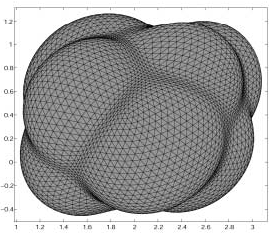
\includegraphics[width=0.4\textwidth]{image/dim01.png}
\caption{Foam rendered by Boundary Integral Method}
\label{fig:dim-foam}
\end{figure}

The transparency is an important aspect of the foam. The transparency can be calculated\cite{nvidia} according to the Equation \ref{equa:transparency}, and apply the acquired value to the geometric primitive used for the foam representation.

\begin{equation}
alpha=saturate(\frac{H-H_0}{H_{max} - H_0})
\label{equa:transparency}
\end{equation}

We can combine the texture with the BIM way of modeling the foam. Apply the texture for further visualization. Since the eye sees a mixed between the colors in long distances, it is possible to apply the texture for saving processing and reduce the aliasing effect.
For a detailed visualization we render the geometric primitive modeled with BIM for the foam.

The foam flow can be computed using two tecniques from dinamical fields (fluid dynamics): surface elevation and potential velocity.

The dynamic aspect of the foam can be modeled using phisically based particle. The particle should respect the gravity, and wind forces until the shore. Based on the elevation of the waves crest defines the speed of the foam. Is possible to use the Gestners model, as in this model we are aware of the wave trajectory, we can follow trajectory and set the very same path for the foam, applying some dispersion to it\cite{iaow}.
The environment conditions for the foam is that the waves must be sufficiently high enough to break and produce the foam(slope greater than 1/6 \cite{sow} of the height of the wave).
When the foam reaches the beach, it should disapear. Removing the particles from outter to the inner layer, simulating the bubble bursted by the wind, since the inner ones are protected the outter bubbles, they tend to burst more easily.

[missing refraction, specular reflaction ]


\begin{thebibliography}{9}

\bibitem{sow}
  Simulating Ocean Water,
  TESSENDORF, Jerry.
  2001

\bibitem{iaow}
  Interactive Animation of Ocean Waves,
  HINSINGER, Damien. NEYRET, Fabrice. CANI, Marie-Paule.
  iMAGIS-GRAVIR

\bibitem{nvidia}
  GPU Gems 2,
  Kryachko,Yuri.
  GPU Gems 2. 
  Second printing, April 2005.
  \url{http://http.developer.nvidia.com/GPUGems2/gpugems2_chapter18.html}

\bibitem{bim}
  Boundary Integral for 3d Simulation of Foam Dynamics,
  Ivan B. Bazhlekov, Frans N. van de Vosse, and Han E.H. Meijer.
  Eindhoven University of Technology.

\end{thebibliography}



\end{document}


